\newpage
\section{Decorator Pattern}

Decorator pattern allows a user to add new functionality to an existing object without altering its structure. This type of design pattern comes under structural pattern as this pattern acts as a wrapper to existing class.

This pattern creates a decorator class which wraps the original class and provides additional functionality keeping class methods signature intact.

We are demonstrating the use of decorator pattern via following example in which we will decorate a shape with some color without alter shape class.

\subsection{Implementation}

We're going to create a Shape interface and concrete classes implementing the Shape interface. We will then create an abstract decorator class ShapeDecorator implementing the Shape interface and having Shape object as its instance variable.

RedShapeDecorator is concrete class implementing ShapeDecorator.

DecoratorPatternDemo, our demo class will use RedShapeDecorator to decorate Shape objects.

\subsection{Class Diagram}

\begin{figure}[h]
\centering
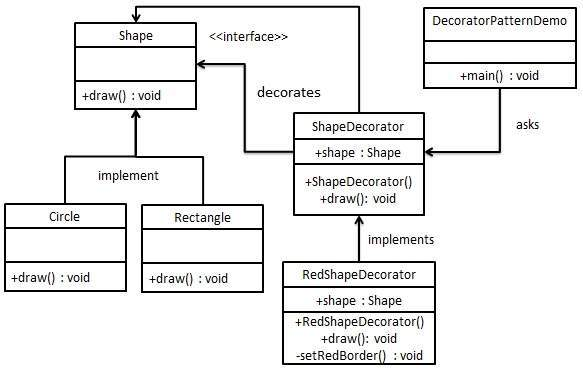
\includegraphics[scale=0.5]{decorator}
\caption{Class Diagram of Decorator Pattern}
\end{figure}

\newpage
\subsection{Source Code (Java)}

\subsubsection{Shape Interface}

\begin{minted}{java}
public interface Shape {
   void draw();
}
\end{minted}

\subsubsection{Rectangle Class}

\begin{minted}{java}
public class Rectangle implements Shape {

   @Override
   public void draw() {
      System.out.println("Shape: Rectangle");
   }
}
\end{minted}

\subsubsection{Circle Class}

\begin{minted}{java}
public class Circle implements Shape {

   @Override
   public void draw() {
      System.out.println("Shape: Circle");
   }
}
\end{minted}

\subsubsection{ShapeDecorator abstract Class}

\begin{minted}{java}
public abstract class ShapeDecorator implements Shape {
   protected Shape decoratedShape;

   public ShapeDecorator(Shape decoratedShape){
      this.decoratedShape = decoratedShape;
   }

   public void draw(){
      decoratedShape.draw();
   }	
}
\end{minted}

\subsubsection{RedShapeDecorator Class}

\begin{minted}{java}
public class RedShapeDecorator extends ShapeDecorator {

   public RedShapeDecorator(Shape decoratedShape) {
      super(decoratedShape);		
   }

   @Override
   public void draw() {
      decoratedShape.draw();	       
      setRedBorder(decoratedShape);
   }

   private void setRedBorder(Shape decoratedShape){
      System.out.println("Border Color: Red");
   }
}
\end{minted}

\subsubsection{Driver Class}

\begin{minted}{java}
public class DecoratorPatternDemo {
   public static void main(String[] args) {

      Shape circle = new Circle();

      Shape redCircle = new RedShapeDecorator(new Circle());

      Shape redRectangle = new RedShapeDecorator(new Rectangle());
      System.out.println("Circle with normal border");
      circle.draw();

      System.out.println("\nCircle of red border");
      redCircle.draw();

      System.out.println("\nRectangle of red border");
      redRectangle.draw();
   }
}
\end{minted}

\subsection{Output}

\begin{minted}{text}
Circle with normal border
Shape: Circle

Circle of red border
Shape: Circle
Border Color: Red

Rectangle of red border
Shape: Rectangle
Border Color: Red
\end{minted}
